\section{Nuha Hanifatul K - 1184085}
\subsection{Definisi Kecerdasan Buatan}
 \hspace{1cm}Artificial Intelligence (AI) merupakan system kecerdasan buatan yang diselipkan pada teknologi dimana akan dikembangkan secara ilmiah. Kecerdasan yang dimaksudkan adalah pada penekanan kemampuan untuk memperoleh pengetahuan yang dapat diterapkan secara langsung. Hal ini dimana kecerdasan bersal dari kata cerdas yang berarti benar tepat dan cepat, sehingga kecerdasan buatan dibuat untuk menghasilkan hasil kesimpulan yang cepat dan tepat. AI sendiri merupakan cabang ilmu computer, pembelajaran, adaptasi dengan sebuah mesin dan perilaku( behavioral).

\subsection{Sejarah dan perkembangan Kecerdasan Buatan}
\hspace{1cm} ada tahun 1956 kecerdasan buatan pertama kali diciptakan. Sedangkan riset tahap awal dari proyrk AI itu terjadi pada tahun 1950, mengeksplorasi topik penyelesaian masalah dan metode simbolik merupakan tujuan pada saat riset awal tersebut.
Selanjutnya Departemen Pertahanan dari Amerika Serikat juga mempunyai keinginan untuk mengembangkan serta melatih computer agar mempunyai penalaran seperti manusia secara dasar hal ini terjadi pada tahun 1960 an. Selanjutnya 10 tahun kemudian yaitu 1970 an telah berhasil proyek pemetaan jalan yaitu proyek DARPA(defence Advanced Research Project Agency). Dan DARPA pula telah berhasil dengan asisten pribadi pada 2003. Hingga sekarang teknologi AI terus berkembang dan selalu dikembangkan untuk dapat memenuhi kebutuhan yang seakin kompleks.

\subsection{Supervised Learning, Klasifikasi, Regresi dan Unsupervised Learning.}
\begin{enumerate}
\item supervised learning : supervised learning dalam Bahasa Indonesia dapat diartikan sebagai pembelajan dengan adanya supervisiornya. Supervisior merupakan label yang ada pada data, label atau tag tersebut merupakan tag atau label yang ditambahkan dalam mechine learning model. Contoh dalam sebuah data film maka ada tag atau label yang dibuat seberti klasifikasi genre film jadi tiap film memiliki tag atau label genre film nya film romen, keluarga atau animasi.
\item Klasifikasi : Klasifikasi adalah penyusunan bersistem pada golongan atau kelompok menurut kaidah atau senuai dengan standar yang diterapkan.
\item Regresi : Salah satu metode untuk menentukan hubungan sebab-akibat antar variable ini merupakan pengertian dari Regresi. Sedangkan padaanalisis regresi sederhana hubungan antar variable tersebut bersifat linier. Serta umumnya analisis regresi tersebut dapat digunakan untuk ramalan atau prediksi. 
\item Unsupervised Learning : Pada Unsupervised Learning clsifikasi tidak menggunakan label melainkan menggunakan kesamaan atribut yang dimiliki dari data tersebut. Hal ini didasarkan karena memungkin adanya data natural input yang tidak memiliki label sehingga dengan Unsupervised Learning dapat diklasifikan dengan kesamaan atribut yang dimiliki data tersebut. Sebagai contoh kita memiliki 5 film tanpa kita tau genre film tersebut maka kita dapat membuat kelompok atau klsifikasi lain setelah kita menonton film tersebut seperti klasifikasi Sangat menarik, menarik, ataupun tidak menarik.
\end{enumerate}

\subsection{Data Set, Training Test, Testing Test}
\begin{enumerate}
    \item Data set : Merupakan kumpulan data yang akan diolah pada machine learning.
    \item Training set : Dapat kita gunakan dalam pembuatan model machine learning
    \item Testing set : Digunakan sebagai pengujian performa dan kebenaran dari timbal balik dalam model machine learning tersebut.
\end{enumerate}

\section{Instalasi}
\begin{enumerate}
    \item Instalasi library scikit dari anaconda dengan pip install -U scikit-learn
    \begin{center}
    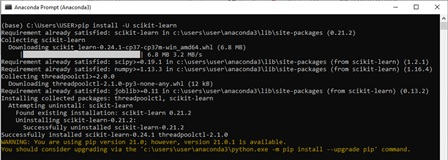
\includegraphics[scale=0.5]{figures/1184085/chapter1/1.jpg}
    \end{center}
    \item Setelah melakukan instalasi kita akan mencoba salah satu example pada web scikit.
    \begin{center}
    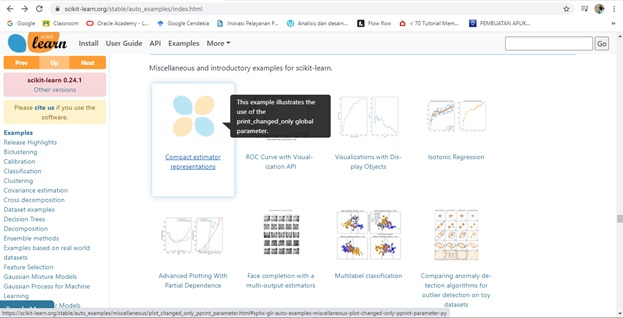
\includegraphics[scale=0.75]{figures/1184085/chapter1/2.jpg}
    \end{center}
    Coba kita copy Paste ke spyder
    \begin{center}
    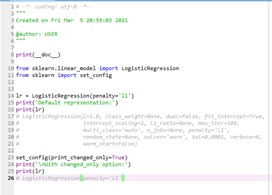
\includegraphics[scale=0.75]{figures/1184085/chapter1/3.jpg}
    \end{center}
    Lalu jalankan dan hasilnya seperti ini.
    \begin{center}
    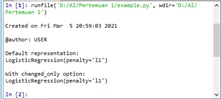
\includegraphics[scale=0.75]{figures/1184085/chapter1/4.jpg}
    \end{center}
    
    \item Selanjutnya kita mencoba Loading an example dataset, dengan membuka website scikit dan menjalankan dengan spyder lalu running untuk melihat hasilnya.
    \begin{center}
    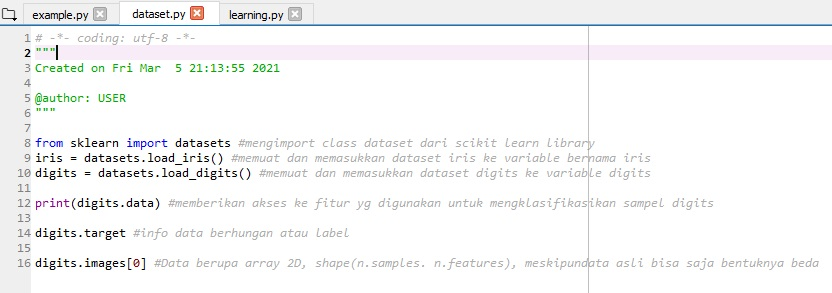
\includegraphics[scale=0.5]{figures/1184085/chapter1/5.jpg}
    \end{center}
    \begin{center}
    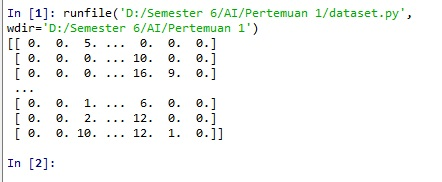
\includegraphics[scale=0.75]{figures/1184085/chapter1/6.jpg}
    \end{center}
    \item Latihan selanjutanya Learning and predicting, dengan membuka website scikit dan menjalankan dengan spyder lalu running untuk melihat hasilnya.
    \begin{center}
    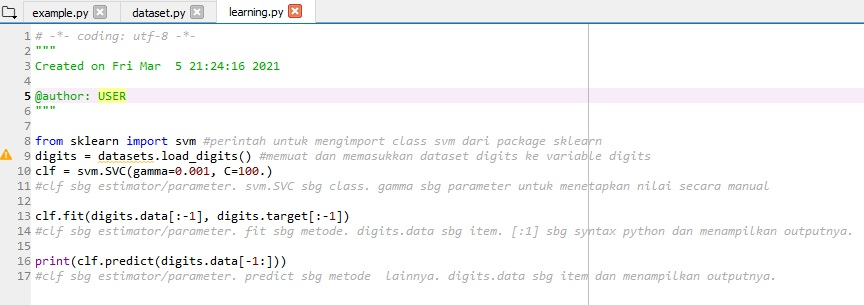
\includegraphics[scale=0.5]{figures/1184085/chapter1/7.jpg}
    \end{center}
    \begin{center}
    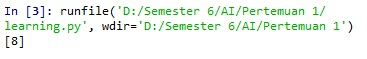
\includegraphics[scale=0.75]{figures/1184085/chapter1/8.jpg}
    \end{center}
    \item Latihan selanjutnya mengenai Model persistence, dengan membuka website scikit dan menjalankan dengan spyder lalu running untuk melihat hasilnya. disini akan menghasilkan file .joblib yang tersimpan di folder yang sama dengan file modelpersisten.py
    \begin{center}
    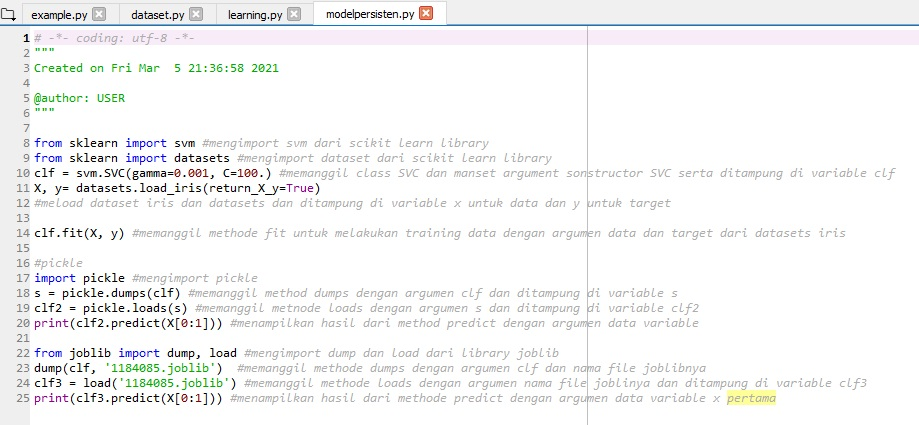
\includegraphics[scale=0.5]{figures/1184085/chapter1/9.jpg}
    \end{center}
    \begin{center}
    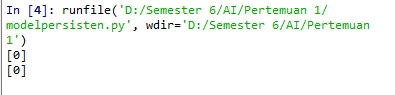
\includegraphics[scale=0.75]{figures/1184085/chapter1/10.jpg}
    \end{center}
    \item Latihan selanjutnya mengenai Conventions, dengan membuka website scikit dan menjalankan dengan spyder lalu running untuk melihat hasilnya.
    \begin{center}
    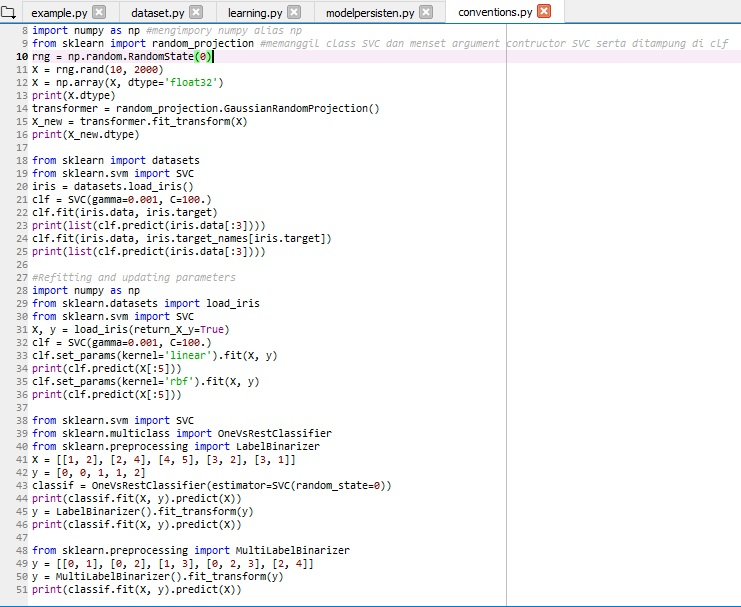
\includegraphics[width=.75\textwidth]{figures/1184085/chapter1/11.jpg}
    \end{center}
    \begin{center}
    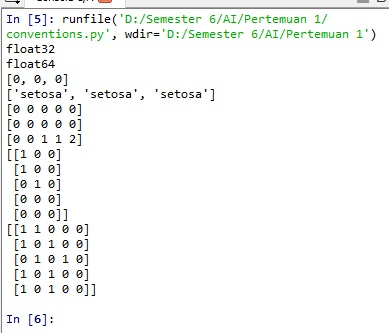
\includegraphics[scale=0.75]{figures/1184085/chapter1/12.jpg}
    \end{center}
\end{enumerate}

\section{Error dan Penanganannya}
\begin{enumerate}
    \item Terdapat error dalam modelpersisten.py yaitu NameError: 'clf3' is not define
    \begin{center}
    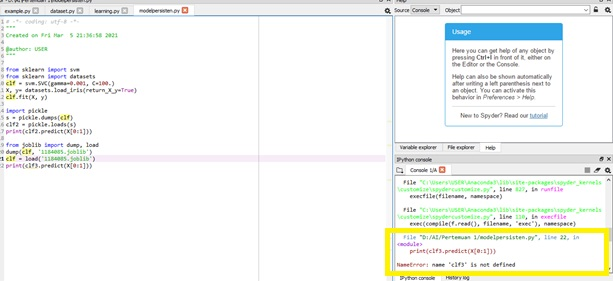
\includegraphics[width=.8\textwidth]{figures/1184085/chapter1/er1.jpg}
    \end{center}
    
    \item Tuliskan Kode dan Jenis eror 
    \par Eror ini terjadi karena saya clf3 belum dideklarasikan sehingga tidak dapat dipanggil.
    
    \item Solusi dan Penangan Eror 
    \par jadi eror ini dapat diselesaikan dengan mendefinisian clf3 di baris kode sebelumnya sehingga dapat dipanggil nantinya. 

\end{enumerate}
